\subsection{Utilización de APIs}
\label{subsecc:Utilización de APIs}

En la aplicación de Baldugenda se ha usado 3 apis principalmente que son la de Google Calendar, Google Drive y la de Splunk Mint.
El api de Google Calendar se ha usado para el manejo de los eventos de examen dentro del calendario de Google y la creación y modificación de dichos eventos.
El api de Google Drive se ha usado para la realización del backup.
Y aunque Google nos proporciona medios para debugear la aplicación y ver qué tipos de dispositivos se la instalan se ha decidido usar el api de splunk mint para esta función ya que ofrece información específica de los errores sin que el usuario que la está usando tenga que mandar nada.

\subsection{Dispositivos}
\label{subsecc:Dispositivos}

Una de los requisitos que tenía que cumplir Baldugenda era que fuera accesible a todo el mundo que usara Android. Ya que es una labor difícil porque hay muchos dispositivos se optó por el mal menor y se fijó la versión de Android más baja posible que no diera problemas y que no quitara muchos usuarios.

La versión usada como mínimo en la aplicación fue la API 10-Gingerbread (2.3.3), según estadísticas de Google realizadas en mayo de 2015 la distribución de las versiones de Android esta así.

\begin{figure}[H] 
  \begin{center} 
    \scalebox{0.4}{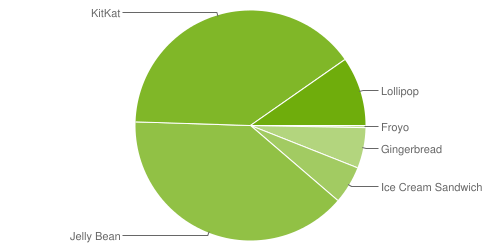
\includegraphics{figs/VersionesAndroid.png}} 
    \caption{Versiones de Android developer.android.com} 
    \label{fig:VersionesAndroid} 
  \end{center} 
\end{figure}

Aparte de la versión se tuvo que decidir para que tipo de pantallas se lanzaría la aplicación, ya que optar por todas haría que la app pesara demasiado.

Se consultó el grafico de pantallas de Google y se decidió dejar fuera la xxhdpi y a la ldpi y usar la mdpi,hdpi y xhdpi

\begin{figure}[H] 
  \begin{center} 
    \scalebox{0.4}{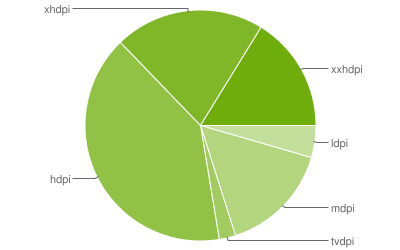
\includegraphics{figs/TiposPantalla.png}} 
    \caption{Tipos de pantalla developer.android.com} 
    \label{fig:TiposPantalla} 
  \end{center} 
\end{figure}

\subsection{Almacenamiento}
\label{subsecc:Almacenamiento}

Para el desarrollo de la aplicación se ha optado por almacenar la información en ficheros sqlite que después el programa leerá y tratara los datos. 
Durante toda la fase de implementación de la aplicación se ha ido modificando la BD hasta llegar a la versión 3 que es la que se está usando actualmente.
En cada una de las versiones se iban añadiendo campos que pedían los Baldusers, y al crear nueva versión de la BD se ha tenido que ir actualizando las BDs creadas ya en los Baldusers que ya se habían instalado la aplicación.
Estas actualizaciones eran referentes a crear columnas nuevas en las tablas o llegando a recorrer las tablas enteras para organizar los datos.
Se ha creado 3 tablas, una para las asignaturas, otra para los exámenes y la última para las notas de los exámenes.

Las tablas tienen las siguientes columnas:
\subsubsection{Asignaturas}
\label{subsubsecc:Asignaturas}


\textbf{Campo id incremental} clave primaria integer

\textbf{Nombre} campo único string, el nombre de la asignatura

\textbf{Enlaces}   un único string donde cada enlace que se presenta esta separado por “;”

\textbf{Evaluación} string que puede tener 2 valores Continua o Conjunta

\textbf{Nota} integer, será el valor máximo que se puede sacar en la asignatura

\subsubsection{Exámenes}
\label{subsubsecc:Exámenes}


\textbf{Campo id incremental} clave primaria integer

\textbf{Nombre} campo único string, el nombre del examen

\textbf{Asignatura} campo único string, el nombre de la asignatura

\textbf{Fecha} campo string, tendrá la fecha en formato DD/MM/AAAA

\textbf{Hora} campo string, tendrá la hora en formato HH:MM

\textbf{Tipo Guardado} campo string, puede tener 2 valores Ambos (si se ha podido crear el evento en Google Calendar) o Local  en caso contrario

\textbf{CalendarioId} campo string, tiene el id donde se ha generado el evento de Google Calendar

\textbf{EventoId} campo string, contiene el valor id del evento para ese examen

\textbf{CalendarioNombre} campo string, nombre del calendario donde se ha generado el evento de Google Calendar

\textbf{Descripción} campo string, descripción del examen

\subsubsection{Notas}
\label{subsubsecc:Notas}


\textbf{Campo id incremental} clave primaria integer

\textbf{Examen} campo único string, nombre del examen

\textbf{Asignatura} campo único string, nombre de la asignatura

\textbf{Nota} campo integer, nota sacada en el examen

\textbf{Nota\_Sobre} campo integer, nota máxima en el examen


Tanto en la tabla de exámenes como en la de notas se ha tenido que especificar que sea un campo único con multi valor para que no se puedan crear exámenes repetidos o duplicar notas.
A la hora de crear la base de datos se crea la BD versión 1 y la aplicación comprueba si había alguna BD en el dispositivo y que versión tiene dependiendo de eso entrara a la función de upgrade que lo que hará es realizar las actualizaciones para actualizar la BD a la versión más actual.

\subsection{Backup}
\label{subsecc:Backup}

Para esta función de Backup se ha usado el api de Google Drive, al usuario se le da la opción de exportar la base de datos a la carpeta que quiera de su Google Drive.
Para exportar primero se realiza una conexión con el servicio de Google se comprueba que tiene los permisos necesarios para realizar la creación de carpetas y ficheros y una vez Google ha mandado la respuesta, se puede acceder al Google Drive mediante una actividad que proporciona el propio api de Google Drive que muestra las carpetas del Drive y da la posibilidad de crear nuevas carpetas. 
Ya que la conexión es  asíncrona se ha tenido que separar la opción de seleccionar la carpeta donde el usuario subirá la base de datos de la opción de subir la base de datos,  si se realizaba junto al intentar subir la BD la aplicación se bloqueaba porque Google todavía no tenía la carpeta creada en su base de datos. 
A la hora de crear el fichero que se sube a Google Drive se ha realizado una transformación de un fichero a bytes.
Y después se han escrito esos bytes en el canal de entrada para el fichero que se deseaba crear.
El fichero coge el nombre de la base de datos y se le añade la fecha y la hora en la que se ha creado el fichero para que el usuario pueda escoger con facilidad ordenándolo por nombre.
Para importar la base de datos lo único que tiene que hacer el usuario es seleccionar el fichero que quiere importar y darle al botón de importar base de datos.
La lógica de negocio se encarga de coger el fichero seleccionado de Google Drive y dirigir el canal de salida del fichero escogido al fichero que se crea en la ruta de la base de datos, que en caso de que exista se borra.

\subsection{Interacción con la app}
\label{subsecc:Interacción con la app}

El manejo de Baldugenda según los Baldusers es sencillo, para acceder a la lista de asignaturas o a la lista de exámenes solo hace falta darle al icono del menú principal.
Aparte de este menú que se basa en icono con títulos que explica para que es cada icono, podemos ver las listas de asignaturas y de exámenes, cada lista tiene cosas únicas que se han colocado para probar acciones dentro de una aplicación Android.
En la lista de asignaturas se puede encontrar un menú de búsqueda para que el usuario en el caso de que tenga muchas asignaturas, escribiendo el nombre de la asignatura en la caja de texto le aparecería esa asignatura en la lista.
Aparte se ha añadido la opción de la pulsación larga en cada asignatura para poder editarla y borrarla.
En la actividad de exámenes se puede ver que la lista no es igual a la lista de asignaturas, se ha usado la clase ExpandableList para crear cajones donde ira la asignatura y los exámenes de esa asignatura, junto con el número de exámenes que hay dentro de la asignatura.
Se ha modificado el botón de atrás dentro de la actividad lista exámenes para que muestre un menú de navegación lateral para poder ir a cualquiera de las actividades mostradas. A los Baldusers les pareció bien el menú pero ninguno vio necesario ponerlo en cada actividad.
